\section{Movimiento Browniano}

%----------------------------------------------------------------------------------------

\begin{frame}
%center the title
    \begin{center}
        \textbf{\huge Movimiento Browniano}
    \end{center}
\end{frame}

%----------------------------------------------------------------------------------------

\begin{frame}
    \frametitle{Procesos Estocásticos}
    \begin{itemize}
        \item Variables que cambian de valor en el tiempo de forma incierta.
        \item Clasificación: tiempo discreto o continuo, variable continua o discreta.
        \item Definición formal: un proceso estocástico es una colección de variables aleatorias indexadas por el tiempo.
        \[X: \Omega \times I \rightarrow \mathbb{R}\]
    \end{itemize}
\end{frame}

%----------------------------------------------------------------------------------------

\begin{frame}
    \frametitle{Definición del Proceso \( S_t(\omega_1 \omega_2 \omega_3) \)}
    
    \[
    S_0(\omega_1 \omega_2 \omega_3) = 4 \quad \text{para todo } \omega_1 \omega_2 \omega_3 \in \Omega_3,
    \]
    
    \[
    S_1(\omega_1 \omega_2 \omega_3) =
    \begin{cases}
        8 & \text{si } \omega_1 = C, \\
        2 & \text{si } \omega_1 = N,
    \end{cases}
    \]
    
    \[
    S_2(\omega_1 \omega_2 \omega_3) =
    \begin{cases}
        16 & \text{si } \omega_1 = \omega_2 = C, \\
        4 & \text{si } \omega_1 \ne \omega_2, \\
        1 & \text{si } \omega_1 = \omega_2 = N,
    \end{cases}
    \]
    
    \[
    S_3(\omega_1 \omega_2 \omega_3) =
    \begin{cases}
        32 & \text{si } \omega_1 = \omega_2 = \omega_3 = C, \\
        8 & \text{si hay dos caras y una cruz}, \\
        2 & \text{si hay una cara y dos cruces}, \\
        0.5 & \text{si } \omega_1 = \omega_2 = \omega_3 = N.
    \end{cases}
    \]

\end{frame}

%----------------------------------------------------------------------------------------

\begin{frame}
    \frametitle{Evolución de $S_t$}
    \begin{figure}
        \centering
        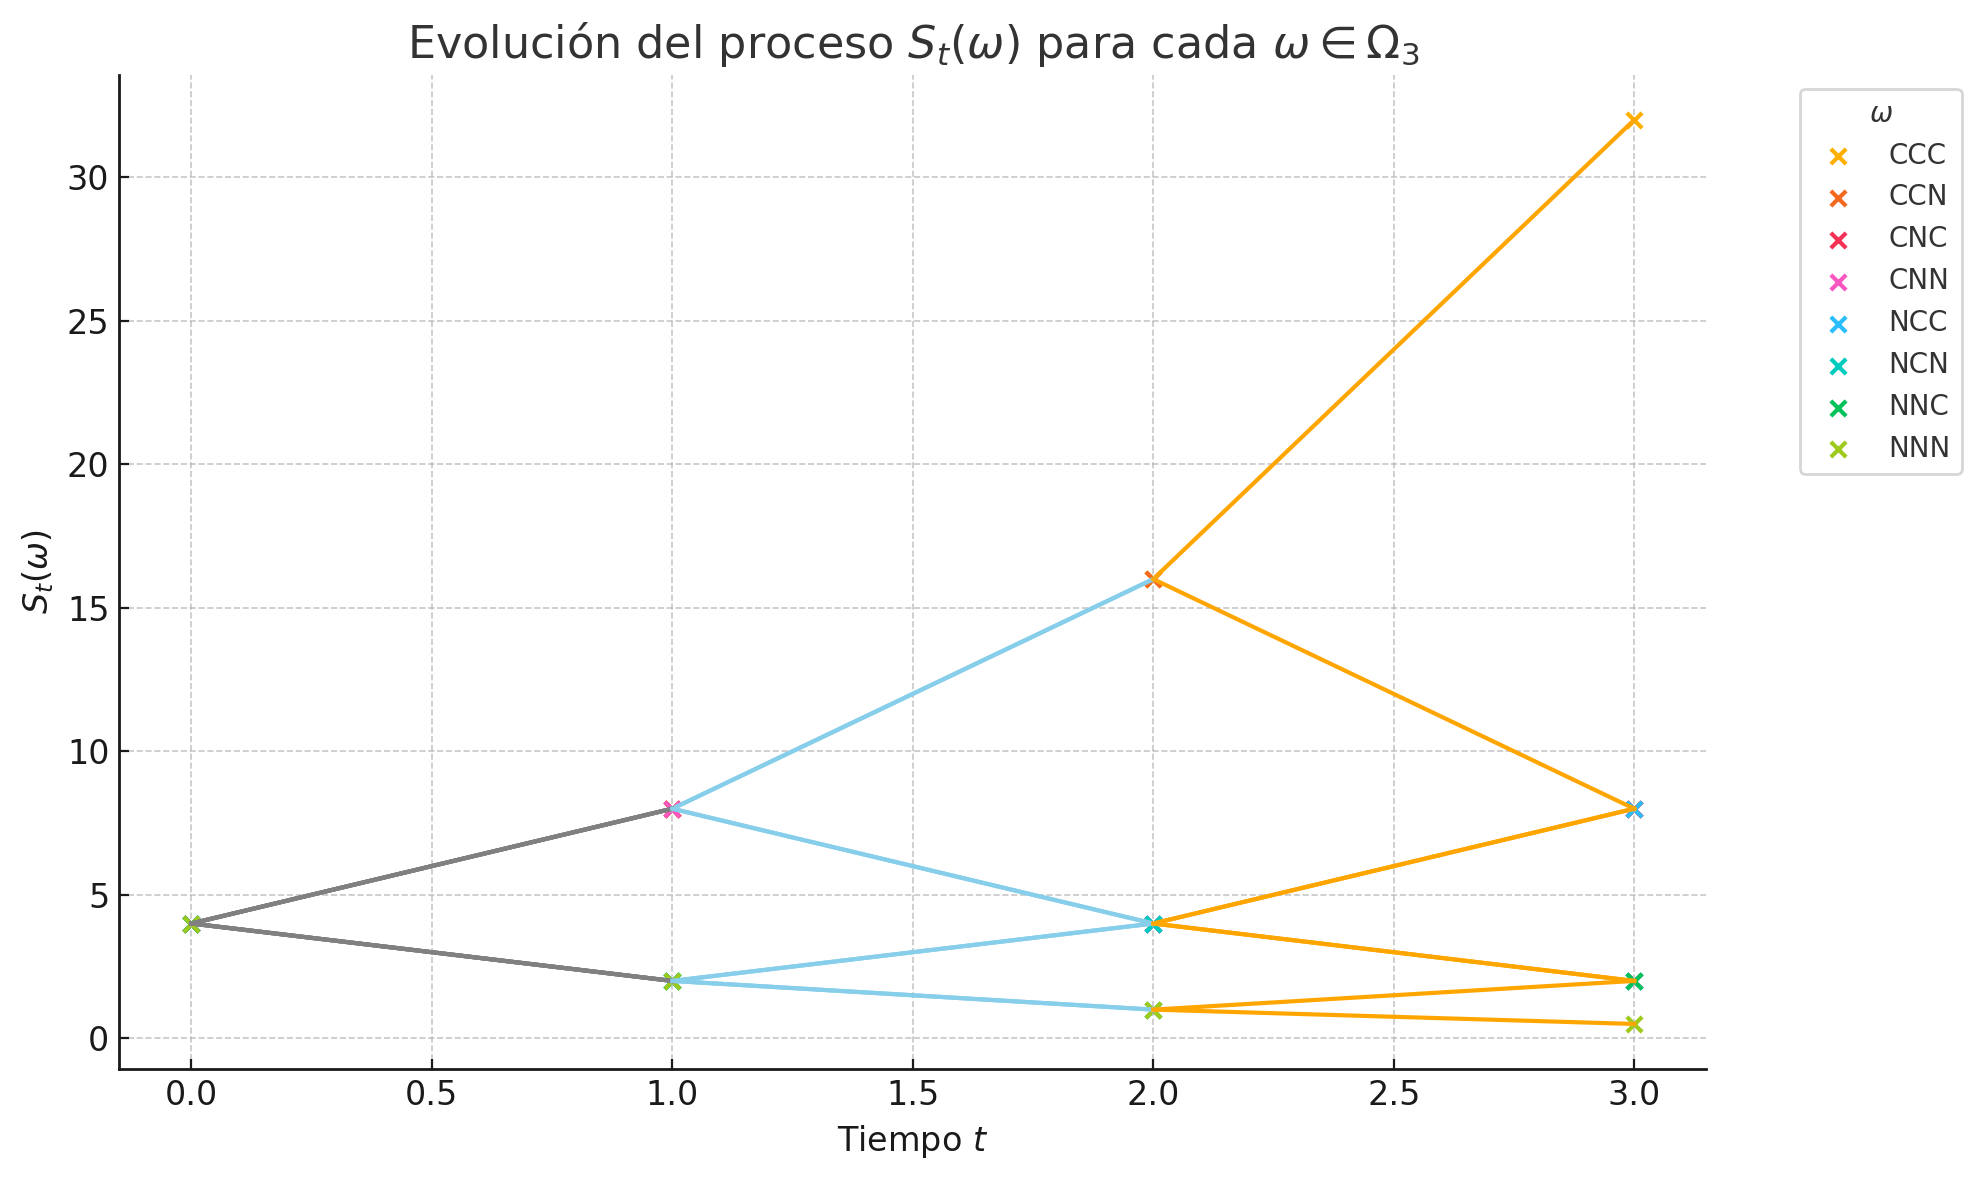
\includegraphics[width=0.8\textwidth]{img/cap2/S_t.jpg}
        \caption{Evolución del proceso $S_t$ en el tiempo.}
        \label{fig:evolucion}
    \end{figure}
\end{frame}

%----------------------------------------------------------------------------------------
\begin{frame}
    \frametitle{Movimiento Browniano}
    \begin{itemize}
        \item Proceso continuo que comienza en 0: \(W(0) = 0\).
        \item Incrementos independientes y distribuidos normalmente.
        \item Propiedades:
        \begin{itemize}
            \item \(\mathbb{E}[W(t)] = 0\).
            \item \(\text{Var}[W(t)] = t\).
        \end{itemize}
    \end{itemize}
\end{frame}

%----------------------------------------------------------------------------------------

\begin{frame}
    \frametitle{Valor Esperado Condicional}
    \begin{itemize}
        \item Definición: \(\mathbb{E}[X|\mathcal{G}]\) satisface medibilidad y promedio parcial.
        \item Propiedades:
        \begin{itemize}
            \item Linealidad.
            \item Condicionamiento iterado.
            \item Desigualdad de Jensen.
        \end{itemize}
    \end{itemize}
\end{frame}

%----------------------------------------------------------------------------------------

\begin{frame}
    \frametitle{Martingalas}
    \begin{itemize}
        \item Proceso estocástico sin deriva.
        \item Propiedad clave: \(\mathbb{E}[M(t)|\mathcal{F}(s)] = M(s)\).
        \item Ejemplo: Movimiento Browniano es una martingala.
    \end{itemize}
\end{frame}

%----------------------------------------------------------------------------------------

\begin{frame}
    \frametitle{Proceso de Itô}
    \begin{itemize}
        \item Modelo para capturar la naturaleza estocástica de los precios de activos financieros.
        \item Representación general:
        \[dX = \mu(X, t) \, dt + \sigma(X, t) \, dW\]
        \item \(\mu\): tasa de deriva. \(\sigma\): volatilidad.
    \end{itemize}
\end{frame}

%----------------------------------------------------------------------------------------

\begin{frame}
    \frametitle{Lema de Itô}
    \begin{itemize}
        \item Relaciona una función \(G(X, t)\) con el proceso de Itô subyacente.
        \item Fórmula:
        \[dG = \frac{\partial G}{\partial t} \, dt + \frac{\partial G}{\partial X} \, dX + \frac{1}{2} \frac{\partial^2 G}{\partial X^2} \, (\sigma^2 \, dt)\]
        \item Aplicación: valuación de derivados financieros.
    \end{itemize}
\end{frame}